%Homework Template
%----------------------------------------
\documentclass[11zpt]{article}
\usepackage[margin=1in]{geometry} 
\usepackage{amsmath,amsthm,amssymb,amsfonts}
\usepackage{ifthen}
\usepackage{pbox}
\usepackage{romannum}
\usepackage{centernot}
\usepackage{color,soul}
\usepackage{pgfplots}


\newenvironment{problem}[2][Problem]{\begin{trivlist}
\item[\hskip \labelsep {\bfseries #1}\hskip \labelsep {\bfseries #2.}]}{\end{trivlist}}
\renewcommand{\qedsymbol}{$\blacksquare$}
\usepackage{fancyhdr}
\usepackage{pst-plot}

%SetFonts
\pagestyle{fancy}
\rhead{Homework 1}
\lhead{Jugal Marfatia}
 
%----------------------------------------
% Assignment Title and Your Name
%----------------------------------------
\title{Homework 1}
\author{Jugal Marfatia \\ \\Macroeconomics-1 \\ }
\date{August 30, 2017}
%----------------------------------------
\begin{document}
\maketitle

%========================================
%	START ANSWERS HERE
%========================================
 
\begin{problem}{1}. \\ \\
\textbf{(a)} $  U'(c_t) = \frac{1}{c_t^\sigma} > 0 \implies $ strictly increasing. (Since $\sigma > 0 $)
\\
\\
Next, $U''(c_t) =-\sigma \frac{1}{c_t^{\sigma-1}} < 0 \implies $ strictly concave. (Since $\sigma > 0 $)
\\
\\And finally $ \lim_{c_t \to 0} \frac{1}{c_t^\sigma} = + \infty$
\\
\\
\\
\textbf{(b)} If $\sigma \leq 0 \implies \sigma \frac{1}{c_t^{\sigma-1}} \geq 0 \implies $ not strictly concave.
\\
\\
Also if $\sigma \leq 0 \implies  \lim_{c_t \to 0} \frac{1}{c_t^\sigma} \neq + \infty$ 
\\
\\
\\
\textbf{(c)} $\lim_{\sigma \to 1} \frac{c_t^{1-\sigma}- 1}{\sigma - 1} = \lim_{\sigma \to 1} \frac{e^{ln(c_t){(1-\sigma)}}- 1}{\sigma - 1} = \lim_{\sigma \to 1} \frac{- e^{\ln(c_t){(1-\sigma)}}\ln(c_t)}{- 1} = \frac{- \ln(c_t)}{- 1} = \ln(c_t)$ 
\\
\\
\\
\textbf{(d)} $U'(c_t) = \frac{1}{c_t^\sigma} $ and $U''(c_t) =-\sigma \frac{1}{c_t^{\sigma-1}} $
\\
\\
Therefore, $ -\frac{c U''(c_t)}{U'(c_t)} = \frac{c c^{\sigma}\sigma}{c^{\sigma+1}} = \sigma $ (a constant). 
\\
\\
\\
\textbf{(e)} $U(c_0, c_1, ..., c_T) = \sum_{t=0}^{T} \beta^t  \frac{c_t^{1- \sigma} - 1}{1-\sigma} = \sum_{t=0}^{T} \beta^t  \frac{c_t^{1- \sigma}}{1-\sigma} - \sum_{t=0}^{T}  \frac{\beta^t }{1-\sigma} $
\\
\\
\\
Let $g(x) = \big[ x +  \sum_{t=0}^{T}  \frac{\beta^t }{1-\sigma} \big]^{\frac{1}{1-\sigma}}$ and $g'(x) = \frac{1}{1-\sigma} \big[ x +  \sum_{t=0}^{T}  \frac{\beta^t }{1-\sigma} \big]^{\frac{1}{1-\sigma}-1} > 0. \implies $ Strictly increasing. 
\\
\\
\\
Therefore, $g(U(c_0, c_1, ..., c_T)) = \big[ \sum_{t=0}^{T} \beta^t  \frac{c_t^{1- \sigma}}{1-\sigma} - \sum_{t=0}^{T}  \frac{\beta^t }{1-\sigma} +  \sum_{t=0}^{T}  \frac{\beta^t }{1-\sigma} \big]^{\frac{1}{1-\sigma}} = \big[ \sum_{t=0}^{T} \beta^t  \frac{c_t^{1- \sigma}}{1-\sigma} \big]^{\frac{1}{1-\sigma}}$ 
\\
\\
\\
And if we set $\alpha^t = \frac{\beta^t }{1-\sigma}$
\\
\\
\\
we get $ g(U(c_0, c_1, ..., c_T)) = \big[ \sum_{t=0}^{T} \alpha^t  c_t^{1- \sigma} \big]^{\frac{1}{1-\sigma}} = \big[ \alpha^0  c_0^{1- \sigma} +  \alpha^1  c_1^{1- \sigma} + ..+  \alpha^T  c_T^{1- \sigma}   \big]^{\frac{1}{1-\sigma}}$
\\
\\
\\
Therefore the utility function is a CES function. 
\\
\\
\\
\\
\textbf{(f)} Since $\lim_{\sigma \to 1} \frac{c_t^{1-\sigma}- 1}{\sigma - 1} = \ln(c_t) 
\\ 
\\
\implies $ when $\sigma = 1, 
\\ 
U(c_0, c_1, ..., c_T) = \sum_{t=0}^{T} \beta^t  \frac{c_t^{1- \sigma} - 1}{1-\sigma} = \sum_{t=0}^{T} \beta^t  \ln(c_t) = \sum_{t=0}^{T}  \ln(c_t^{\beta^t}) = \big[\ln(c_0^{\beta^0}) + \ln(c_1^{\beta^1}) + ....+ \ln(c_T^{\beta^T}) \big]$
\\
\\
\\
Next let $ g(x) = e^x $ and $g'(x) = e^x > 0 \implies $ (Strictly increasing)
\\
\\
\\
Therefore, $g(U(c_0, c_1, ..., c_T)) =  e^{\big[\ln(c_0^{\beta^0}) + \ln(c_1^{\beta^1})+ ...+ \ln(c_T^{\beta^T}) \big]} = e^{\big[\ln(c_0^{\beta^0} c_1^{\beta^1} ... c_T^{\beta^T}) \big]} = c_0^{\beta^0} c_1^{\beta^1} .... c_T^{\beta^T}$
\\
\\
\\
Thus the utility function is a Cobb Douglas function when $\sigma = 1 $. 
\\
\\
\\
\\
\textbf{(g)} We will use the result from e. i.e. $ g(U(c_0, c_1, ..., c_t)) = \big[ \alpha^0  c_0^{1- \sigma} +  \alpha^1  c_1^{1- \sigma} + ..+  \alpha^T  c_T^{1- \sigma}   \big]^{\frac{1}{1-\sigma}} $
\\ 
\\
Therefore, 
\\
\begin{flalign*} 
 g(U(\beta c_0, \beta c_1, ..., \beta c_T)) & = \big[ \alpha^0  ( \beta c_0)^{1- \sigma} +  \alpha^1  (\beta c_1)^{1- \sigma} + ..+  \alpha^T  (\beta c_T)^{1- \sigma}   \big]^{\frac{1}{1-\sigma}}  & \\ \\
              & = \big[ \alpha^0   \beta^{1- \sigma} c_0^{1- \sigma} +  \alpha^1  \beta^{1- \sigma} c_1^{1- \sigma} + ..+  \alpha^T  \beta^{1- \sigma} c_T^{1- \sigma}   \big]^{\frac{1}{1-\sigma}} & \\ \\
              & = \beta^{\frac{1- \sigma}{1- \sigma}}\big[ \alpha^0   c_0^{1- \sigma} +  \alpha^1   c_1^{1- \sigma} + ..+  \alpha^T  c_T^{1- \sigma}   \big]^{\frac{1}{1-\sigma}} & \\ \\
              & = \beta \big[ \alpha^0   c_0^{1- \sigma} +  \alpha^1   c_1^{1- \sigma} + ..+  \alpha^T  c_T^{1- \sigma}   \big]^{\frac{1}{1-\sigma}} & \\ \\
              & = \beta g(U( c_0,  c_1, ..., c_t))
\end{flalign*} 
\\
\\
Thus $ g(U(\beta c_0, \beta c_1, ..., \beta c_T)) = \beta g(U( c_0,  c_1, ..., c_t)) \implies U(c_0, c_1, ..., c_T) $ is homothetic. 
\\
\\
\end{problem}
\pagebreak
\begin{problem}{2}. \\ \\
\textbf{(a)} 
\begin{flalign*} 
F(tk, tn) & = A \big[ \alpha (tk)^{1-\sigma}  + (1-\alpha) (tn)^{1-\sigma} \big]^{\frac{1}{1-\sigma}} & \\ \\
              & = A \big[ (t^{1-\sigma}) (\alpha k^{1-\sigma}  + (1-\alpha) n^{1-\sigma}) \big]^{\frac{1}{1-\sigma}} & \\ \\
              & =t^{\frac{1-\sigma}{1-\sigma}} A \big[  (\alpha k^{1-\sigma}  + (1-\alpha) n^{1-\sigma} \big]^{\frac{1}{1-\sigma}} & \\ \\
              & =t A \big[  (\alpha k^{1-\sigma}  + (1-\alpha) n^{1-\sigma} \big]^{\frac{1}{1-\sigma}} & \\ \\
              & =t F(k, n)
\end{flalign*} 
\\
Therefore, $F(tk, tn) = t F(k, n)$  
\\
\\
\\
\textbf{(b)} As hinted in the question we will first take the log of the equation in order to find the limit.
\begin{flalign*}
\log(F(k, n)) & = \log(A) + \frac{1}{1-\sigma} \log \big[ \alpha (k)^{1-\sigma}  + (1-\alpha) (n)^{1-\sigma} \big]  & \\ \\ 
\therefore \lim_{\sigma \to 1} \log(F(k, n)) & = \log(A) + \lim_{\sigma \to 1} \frac{\log \big[ \alpha (k)^{1-\sigma}  + (1-\alpha) (n)^{1-\sigma} \big]}{1-\sigma}  & \\ \\
            & =\log(A) + \lim_{\sigma \to 1} \frac{-\big[ \alpha \log(k) e^{\log(k){(1-\sigma)}}  + (1-\alpha)\log(n) e^{\log(n){(1-\sigma)}} \big]}{-\big[ \alpha (k)^{1-\sigma}  + (1-\alpha) (n)^{1-\sigma} \big]}  & \text{(L'Hopitals rule) }  \\ \\
           & =\log(A) + \big[ \alpha \log(k)  + (1-\alpha) \log(n)  \big]  &  \\ \\
\implies  \lim_{\sigma \to 1} \log(F(k, n)) & =\log(A k^\alpha n^{1-\alpha})
\end{flalign*} 
\\
Therefore, $\lim_{\sigma \to 1} e^{\log(F(k, n))}  =e^{\log(A k^\alpha n^{1-\alpha})} \iff  \lim_{\sigma \to 1} F(k, n) =  A k^\alpha n^{1-\alpha} $ 
\\
\\
\\
\textbf{(c)}. 
\\
\\
$F_k(k,n) = A n^{1-\alpha} \alpha k^{\alpha - 1} = \frac{A n^{1-\alpha} \alpha }{k^{1- \alpha }}  > 0 $ ( Since all terms are $> 0$ )
\\
\\
$F_n(k,n) = \frac{ A (1- \alpha) k^{\alpha }}{n^\alpha} > 0 $ ( Since all terms are $> 0 $ ) 
\\
\\
$\lim_{k \to 0 } \frac{A n^{1-\alpha} \alpha }{k^{1- \alpha }} = \frac{A n^{1-\alpha} \alpha }{\lim_{k \to 0 }  k^{1- \alpha }} = \infty$
\\
\\
$\lim_{k \to \infty } \frac{A n^{1-\alpha} \alpha }{k^{1- \alpha }} = \frac{A n^{1-\alpha} \alpha }{\lim_{k \to \infty }  k^{1- \alpha }} = 0$
\\
\\
\\
\\
\textbf{(d)}. 
\\
\\
$\frac{F_k(k,n)k}{F(k,n)} = \frac{ A n^{1-\alpha} \alpha (k^{\alpha - 1}) k}{ A n^{1-\alpha}  (k^{\alpha})}  = \alpha $ 
\\
\\
\\
$\frac{F_n(k,n)n}{F(k,n)} = \frac{ A (1- \alpha) k^{\alpha }n^{1-\alpha}}{A n^{1-\alpha}  (k^{\alpha})} = (1- \alpha) $
\\
\\
\end{problem}
\begin{problem}{3}. \\ \\
\textbf{(a)}. We have $k_{t+1} = s(k_t) F(k_t,1)+ (1-\delta) k_t $ 
\\
\\
Further since $s(k_t) = \bar{s}$,  $  F(k_t, 1) = k_t^\alpha $
\\
\\
$k_{t+1} = \bar{s} k_t^\alpha + (1-\delta) k_t $ \\ 
\\
$ \frac{dk_{t+1}}{dk_t} = \alpha \bar{s} k_t^{\alpha -1 }  + (1-\delta)  > 0 \implies $ strictly increasing (Since all terms are $ > 0 $ and given $\alpha \in (0,1). $)
\\ 
\\
$ \frac{d^2k_{t+1}}{dk_t^2} = \alpha (\alpha -1)$ $  \bar{s}$ $ k_t^{\alpha -2 }  < 0 \implies$ strictly concave (Given $\alpha \in (0,1). )$ 
\\
\\
Further when $ k_t = 0 \implies  k_{t+1} = 0$ 
\\
\\
There there $ \exists ! k^ * > 0 $  and below is the graphical representation. 
\\
\\\pgfplotsset{width=12cm,compat=1.9}
\begin{tikzpicture}
\begin{axis}[
    axis lines = left,
    xlabel = $k_t$,
    ylabel = {$k_{t+1}$},
    yticklabels={,,},
    xticklabels={,,}
]
%Below the red parabola is defined

%Here the blue parabloa is defined
\addplot [
    domain=0:20, 
    samples=100, 
    color=blue,
    ]
    {3*x^.5};
\addlegendentry{$\bar{s} k_t^\alpha + (1-\delta) k_t $}
\addplot [
    domain=0:20, 
    samples=100, 
    color=black,
]
{x};
\end{axis}
\foreach \Point/\PointLabel in {(4.6,3.87)/k^*}
    \draw[fill=black] \Point circle (0.1) node[above left] {$\PointLabel$};
     \foreach \Point/\PointLabel in {(3.5,3.5)/ \text{When } k_0 < k^*, (9,4.5)/ \text{When } k_0 > k^*}
    \draw[fill=black] \Point circle (0) node[above left] {$\PointLabel$};
    \draw (0,0)+(0:0.9) arc(0:42:0.9);
    \node at (22.5:0.6) {$45^\circ$};
\end{tikzpicture}
\\
\\
\\
\textbf{(b)} Since $s(k_t) =\beta k_t^{1-2\alpha}$ and  $  F(k_t, 1) = k_t^\alpha $
\\
\\
$k_{t+1} = \beta k_t^{1-2\alpha} k_t^\alpha + (1-\delta) k_t = \beta k_t^{1-\alpha} + (1-\delta) k_t$ \\ 
\\
$ \frac{dk_{t+1}}{dk_t} = (1- \alpha )$ $ \beta $ $ k_t^{- \alpha }  + (1-\delta)  > 0 \implies $ strictly increasing (Since all terms are $ > 0 $ and given $\alpha \in (0,1). $)
\\ 
\\
$ \frac{d^2k_{t+1}}{dk_t^2} = -\alpha (1 - \alpha)$  $ k_t^{-\alpha -1 }  < 0 \implies$ strictly concave (Given $\alpha \in (0,1). )$ 
\\
\\
Further when $ k_t = 0 \implies  k_{t+1} = 0$ 
\\
\\
There there $ \exists ! k^ * > 0 $  and below is the graphical representation. 
\\
\\
\pgfplotsset{width=12cm,compat=1.9}
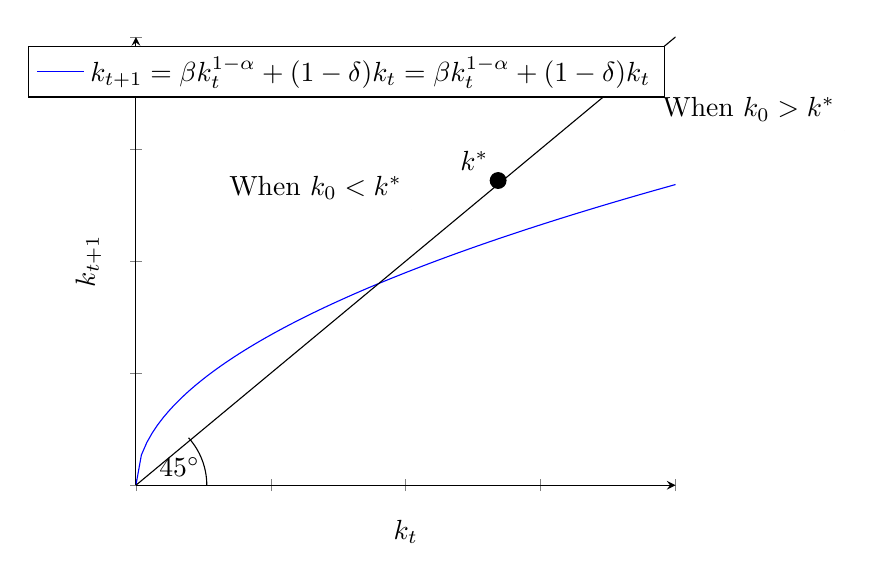
\begin{tikzpicture}
\begin{axis}[
    axis lines = left,
    xlabel = $k_t$,
    ylabel = {$k_{t+1}$},
    yticklabels={,,},
    xticklabels={,,}
]
%Below the red parabola is defined

%Here the blue parabloa is defined
\addplot [
    domain=0:20, 
    samples=100, 
    color=blue,
    ]
    {3*x^.5};
\addlegendentry{$k_{t+1} = \beta k_t^{1-\alpha} + (1-\delta) k_t = \beta k_t^{1-\alpha} + (1-\delta) k_t$}
\addplot [
    domain=0:20, 
    samples=100, 
    color=black,
]
{x};
\end{axis}
\foreach \Point/\PointLabel in {(4.6,3.87)/k^*}
    \draw[fill=black] \Point circle (0.1) node[above left] {$\PointLabel$};
     \foreach \Point/\PointLabel in {(3.5,3.5)/ \text{When } k_0 < k^*, (9,4.5)/ \text{When } k_0 > k^*}
    \draw[fill=black] \Point circle (0) node[above left] {$\PointLabel$};
    \draw (0,0)+(0:0.9) arc(0:42:0.9);
    \node at (22.5:0.6) {$45^\circ$};
\end{tikzpicture}
\\
\\
\\
\textbf{(c)} .
Since $s(k_t) =\beta k_t^{1-\alpha}$ and  $  F(k_t, 1) = k_t^\alpha $
\\
\\
$k_{t+1} = \beta k_t^{1-\alpha} k_t^\alpha + (1-\delta) k_t = \beta k_t^ + (1-\delta) k_t$ \\ 
\\
$ \frac{dk_{t+1}}{dk_t} = $ $ \beta $ $ + 1-\delta > 0 \implies $ Strictly increasing. 
\\
\\
$ \frac{d^2k_{t+1}}{dk_t^2} = 0 \implies $linear and below is the graphical representation. 
\\\\
\\
\pgfplotsset{width=12cm,compat=1.9}
\begin{tikzpicture}
\begin{axis}[
    axis lines = left,
    xlabel = $k_t$,
    ylabel = {$k_{t+1}$},
    yticklabels={,,},
    xticklabels={,,}
]
%Below the red parabola is defined
%Here the blue parabloa is defined
\addplot [
    domain=0:8, 
    samples=100, 
    color=blue,
    ]
    {.5*x};
\addlegendentry{$\delta < \beta $}
\addplot [
    domain=0:5, 
    samples=100, 
    color=red,
    ]
    {2*x};
\addlegendentry{$\delta > \beta$}
\addplot [
    domain=0:8, 
    samples=100, 
    color=black,
]
{x};
\addlegendentry{$\delta = \beta$}
\end{axis}
    \draw (0,0)+(0:0.9) arc(0:42:0.9);
    \node at (22.5:0.6) {$45^\circ$};
\end{tikzpicture}
\\
\\
\textbf{(d)} Since $s(k_t) =\beta k_t^{1-\alpha/2}$ and  $  F(k_t, 1) = k^\alpha $
\\
\\
$k_{t+1} = \beta k_t^{1-\alpha/2} k_t^\alpha + (1-\delta) k_t = \beta k_t^{1+\alpha/2} + (1-\delta) k_t$ \\ 
\\
$ \frac{dk_{t+1}}{dk_t} = (1-\alpha/2)\beta $ $ k_t^{ \alpha/2 }  + (1-\delta)  > 0 \implies $ strictly increasing (Since all terms are $ > 0 $ and given $\alpha \in (0,1). $)
\\ 
\\
$ \frac{d^2k_{t+1}}{dk_t^2} = (1-\alpha/2)(\alpha/2)$  $ k_t^{\alpha/2 -1 }  > 0 \implies$ strictly convex (Given $\alpha \in (0,1). )$ 
\\
\\
Further when $ k_t = 0 \implies  k_{t+1} = 0$ 
\\
\\
There there $ \exists ! k^ * > 0 $  and below is the graphical representation. 
\\
\\\\
\\
Below is the graphical representation. 
\\
\\
\pgfplotsset{width=12cm,compat=1.9}
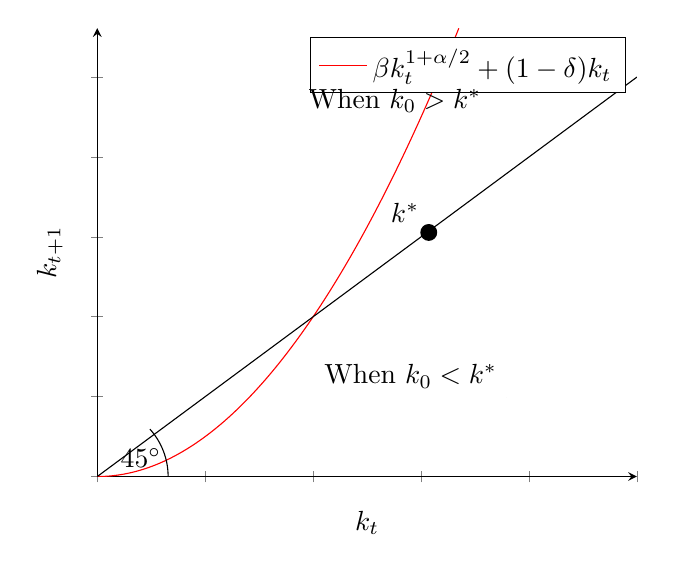
\begin{tikzpicture}
\begin{axis}[
    axis lines = left,
    xlabel = $k_t$,
    ylabel = {$k_{t+1}$},
    yticklabels={,,},
    xticklabels={,,}
]
\addplot [
    domain=0:6.7, 
    samples=100, 
    color=red,
    ]
    {.25*(x^2)};
\addlegendentry{$\beta k_t^{1+\alpha/2} + (1-\delta) k_t$}
\addplot [
    domain=0:10, 
    samples=100, 
    color=black,
]
{x};
\end{axis}
\foreach \Point/\PointLabel in {(4.21,3.1)/k^*}
    \draw[fill=black] \Point circle (0.1) node[above left] {$\PointLabel$};
         \foreach \Point/\PointLabel in {(5.2,1)/ \text{When } k_0 < k^*, (5,4.5)/ \text{When } k_0 > k^*}
    \draw[fill=black] \Point circle (0) node[above left] {$\PointLabel$};
    \draw (0,0)+(0:0.9) arc(0:42:0.9);
    \node at (22.5:0.6) {$45^\circ$};
\end{tikzpicture}
\\
\\
\textbf{(e)} In order to have a unique $k^* > 0$ we need $g(k_t)$ strictly concave or strictly convex and $g(0) = 0 $.\\
\\
Further the saving function $ s(k_t) > 0$  and $ s'(k_t) \geq 0 $
\\
\\
\end{problem}
\begin{problem}{4}.
\\
\\
\textbf{(a)} From the question we have $(1+ g) k_{t+1} = k_t - \delta k_t + i_t $ and since $ i_t - \delta k_t = s_\alpha y_t \implies (1+ g) k_{t+1} = k_t + s_\alpha y_t $
\\
\\
We get $ (1 + g) k^* = k^* + s_\alpha y_t  \iff g k^* =  s_\alpha y_t \iff  k^* =  \frac{s_\alpha y_t}{g}$
\\
\\
Therefore, $\frac{k^*}{y^*} = \frac{s_\alpha}{g} \implies $ if growth rate $ (g) $ decreases to 0 $\frac{k^*}{y^*} $ will approach infinity given $s_\alpha > 0 $. The economic intuition is that if the economy stops growing wages stay constant and the value of the existing capital rises.  
\\
\\
\textbf{(b)} $\frac{r^* k^*}{y^*} = \frac{r s_\alpha}{g} \implies $ if growth rate $ (g) $ decreases to 0 the capital income share $\frac{r^* k^*}{y^*} $ will approach infinity. The economic intuition follows the one in part a and since capital is more valuable it will yield a much higher return compared to wages. 
\\
\\
\\
\textbf{(c)}We have $(1+ g) k_{t+1} = (1 - \delta) k_t + i_t $ and since $ i_t  = s_b y_t \implies (1+ g) k_{t+1} = (1 - \delta) k_t + s_b y_t. $
\\
\\
$\therefore  (1 + g) k^* = (1 - \delta) k^* + s_b y_t \iff (g + \delta) k^* =  s_b y_t \iff  k^* =  \frac{s_\alpha y_t}{(g + \delta)}$
\\
\\
Therefore, $\frac{k^*}{y^*} = \frac{s_b}{(g + \delta)} \implies $ if growth rate $ (g) $ decreases to 0 $\frac{k^*}{y^*} $, unlike the case in part a, will not approach infinity given $ \delta \neq 0$. Furthermore, the  capital income share $\frac{r^* k^*}{y^*} $ will not approach infinity.
\end{problem}
\end{document}
